\documentclass{article}
\setlength{\oddsidemargin}{0.25 in}
\setlength{\evensidemargin}{-0.25 in}
\setlength{\topmargin}{-0.6 in}
\setlength{\textwidth}{6.5 in}
\setlength{\textheight}{8.5 in}
\setlength{\headsep}{0.75 in}
\setlength{\parindent}{0 in}
\setlength{\parskip}{0.1 in}

% ===== PACKAGES =====
\usepackage{amsmath,amssymb}
\usepackage{color}
\usepackage{graphicx}
\usepackage{subfigure}
\usepackage{mdframed}
\usepackage{changepage}
\usepackage[title]{appendix}
\usepackage{hyperref} 
\usepackage{enumitem}
\usepackage{float}
\newmdenv[
  topline=false,
  bottomline=false,
  skipabove=\topsep,
  skipbelow=\topsep
]{siderules}
\renewcommand{\abstractname}{}
\usepackage{listings}
\usepackage{color}
\usepackage{soul}
\definecolor{dkgreen}{rgb}{0,0.6,0}
\definecolor{gray}{rgb}{0.5,0.5,0.5}
\definecolor{mauve}{rgb}{0.58,0,0.82}

\lstset{frame=tb,
  language=Python,
  aboveskip=3mm,
  belowskip=3mm,
  showstringspaces=false,
  columns=flexible,
  basicstyle={\small\ttfamily},
  numbers=none,
  numberstyle=\tiny\color{gray},
  keywordstyle=\color{blue},
  commentstyle=\color{dkgreen},
  stringstyle=\color{mauve},
  breaklines=true,
  breakatwhitespace=true,
  tabsize=3
}

% ===== VARIABLES =====
\def \R{\mathbb{R}}
\def \Pr{\mathbb{P}}
\def \D{{\rm D}}
\def \N{{\rm N}}
\def \xx{{\boldsymbol{\rm x}}}
\def \y{{\rm y}}




% ===== HEADER BOX =====
\newcommand{\lecture}[2]{
\pagestyle{myheadings}
\thispagestyle{plain}
\newpage
\noindent
\begin{center}
\rule{\textwidth}{1.6pt}\vspace*{-\baselineskip}\vspace*{2pt} % Thick horizontal line
\rule{\textwidth}{0.4pt}\\[1\baselineskip] % Thin horizontal line
\vbox{\vspace{2mm}
\hbox to 6.28in { {\bf CS 760: Machine Learning} \hfill Fall 2020 }
\vspace{4mm}
\hbox to 6.28in { {\Large \hfill #1  \hfill} }
\vspace{4mm}
\hbox to 6.28in { {\scshape Authors:}  #2 \hfill }}
\vspace{-2mm}
\rule{\textwidth}{0.4pt}\vspace*{-\baselineskip}\vspace{3.2pt} % Thin horizontal line
\rule{\textwidth}{1.6pt}\\[\baselineskip] % Thick horizontal line
\end{center}
\vspace*{4mm}
}
\bibliographystyle{elsarticle-num}


% =============== DOCUMENT ===============
\begin{document}
\lecture{Predicting female literacy rate and school dropout rate in India }{Bhagyashree Prabhune (bprabhune@wisc.edu) and Saketh Sridhara (ssridhara@wisc.edu)}

\vspace{-4mm}
\begin{abstract}
\textbf{Abstract}:The motivation for this project was to understand one of the key reasons behind the low literacy rate(i.e., high dropout rates amongst schoolchildren) in India. This project aims to predict the dropout rates and enrollment rates among schoolchildren in India, taking into account the large amount of state-wise and district (county) level data collected over a variety of parameters of the current Indian education system. First off, we work with state-wise data over three years of the Indian education system. We identify key features pertaining to the schools, and predict the dropout rates from these features through the linear regression technique. It is seen that the most significant feature is the enrollment rate i.e, higher the enrollment in a state, lower is the dropout rate. For any given feature vector input, the confidence interval for the dropout rate is also established.
Next, having identified enrollment rate as the most important factor for increasing the literacy rate (i.e.  reducing dropouts), we develop a linear regression model which predict enrollment rates from various parameters at the district level (using a larger dataset). We find that the most significant feature affecting the enrollment in schools as the female literacy rate of the district.  Further, the female literacy rates were predicted using SVM, random forest and neural networks. All these ML techniques are in agreement and predicted similar female literacy rate for a feature vector. Also, the significant features affecting female literacy rates are availability of electricity and number of schools with only one teacher. By providing access to electricity and converting the schools from single to multiple teacher schools can help bolster the primary education system of India. This helps states and districts focus on improving the identified resources/infrastructure, which would result in driving up literacy and reducing dropouts. The enrollment and dropout predicting programs can also be utilized to set targets for each district/state in the country. 
  
\end{abstract}

\section{Introduction}

India is a country of 1.3 billion people, where 67\% of the Indian population lives in rural areas. Approx. 196 million elementary school going children, out of that 146 million are enrolled in rural schools (Source: U-DISE 15-16). The school education in rural India is mostly dependent on Government and Government aided schools. For rural India journey of education is not easy, children from rural areas face many challenges till they finish their education.  
The top challenges faced by schoolchildren are - 
  \setlist{nolistsep}
\begin{enumerate}[noitemsep]
\item Lack of electricity and drinking water in schools
\item Lack of proper sanitation facilities (for boys and girls)
\item Lack of an access to computers and advanced learning tools (digital literacy tools)
\item Lack of good infrastructure such as roads and playgrounds
\item Lack of teachers and classroom facilities
\end{enumerate}
And more. These challenges deter children from completing their schooling, and hence they dropout, or worst case, don't enroll to schools. Due to dropouts and reduced enrollments, India's literacy rate stands at about \href{https://data.worldbank.org/indicator/SE.ADT.LITR.ZS?locations=IN} {74\%}. Lower literacy can have detrimental effects on the society, such as increased crime rates, unemployment etc. Hence, it is of utmost importance for a country like India to drive up the enrollment to schools and reduce the droputs. The project aims at using Machine Learning methods to predict dropout rates and enrollment rates based on datasets collected at the state-level and district level across India. The features of the dataset correspond closely the to challenges listed above, and the response we predict are the dropout rates and enrollment rates. 

\href{https://www.indiatoday.in/education-today/featurephilia/story/challenges-of-rural-students-in-india-1703143-2020-07-22}{Link} to the news article from where a portion of this introduction has been adopted. 

\section{Related/Similar work}
Dropout rates have been predicted using machine learning techniques, albeit in a different setting, typically for online learning (where dropout rates were found to be significantly high). Kloft et.al \cite{kloft2014predicting} predicted the dropout rates in MOOC over weeks using Support Vector Machines. Kotsiantis et al. \cite{kotsiantis2003preventing} predicted preventing student dropouts in distance learning using Naive Bayes algorithm. Tan et al. \cite{tan2015prediction} studied high dropout rates in E-learning programs, and developed prediction models using Neural Networks, Decision Trees and Bayesian Networks with a large sample of over 60,000 students, and concluded while all the three methods were effective in prediction, decision tress gave the best performance. Lykourentzou et. al. \cite{lykourentzou2009dropout} using a combination of SVM, Neural Nets and a probabilistic ensemble simplified fuzzy ARTMAP to predict dropout rates for e-learning courses. Fetler et. al. \cite{fetler1989school}, correlated dropout rates, academic performance and poverty using various study variables in the late 80's. The biggest takeaway from literature review was that most ML methods were doing a reasonable job in prediction of dropout rates. We intend to apply a couple of ML techniques and report their accuracy in predicting dropout rates and enrollment rates among schoolchildren in India. 

We are demonstrating variety of ML methods on the data set containing primary education related information from India to make inferences which can aid in it's improvement. 

\section{Dataset}

The aim of this project was to get insights into the dropout and enrollment rates among schoolchildren in India. Hence, we have picked up two relevant datasets, one of which was useful in predicting dropout rates and the other in predicting enrollment rates.

We obtained both the datasets through Kaggle, which have obtained information from the Govt. of India's website \href{https://data.gov.in/}{https://data.gov.in/}. 

The smaller dataset \href{https://www.kaggle.com/vidyapb/indian-school-education-statistics}{State-level dataset} consists of three years of school performance data across the states, and has a total of about 110 data-entries. For the purpose of predicting the dropout rates, a random category of students was chosen (in this case, Secondary Boys), and the entries corresponding to this category was extracted. Missing data was populated with average school data across all categories. All the data is in percentage, hence it is in the same scale. The corresponding CSV file can be found  \href{https://uwprod-my.sharepoint.com/:x:/g/personal/ssridhara_wisc_edu/Ebu49ou21lVCi4geyN82jpkBzErhT8QkI6XciYx0ed4Cag?e=ExgZ3z}{here.} 

The larger dataset \href{https://www.kaggle.com/rajanand/education-in-india}{District-level dataset} contains over school information data from over 600 districts in India. This was used for the analysis on enrollment rates and Female literacy. The corresponding CSV file can be found \href{https://uwprod-my.sharepoint.com/:u:/g/personal/ssridhara_wisc_edu/ERE1fkFjT1tPvzMqik46o1UBbDBkdWNj7p3jxP4TITbzuw?e=UcE0cs}{here}

\section{Approach}
The smaller state-level dataset was used to predict the dropout rates, and the larger district-level dataset was used to predict the enrollment rates. 
With the smaller dataset, dropout rates was predicted using the linear regression model. With the larger dataset, enrollment rates was predicted,  using linear regression model. By analyzing the results obtained through linear regression, we found that female literacy rate is the most significant feature affecting the enrollment rates. Hence the female literacy rate was predicted using support vector machine (SVM), random forest (RF) and neural networks (NN). 

\subsection{Predicting dropout rates using linear regression}
\label{sec:4.1}

The features in the state-level dataset are: The enrollment rates and percentage of schools with computers, toilets , electricity and drinking water supply
The response was chosen to be the dropout ratio. 

First, a heatmap was created to visualize the correlation between the features and the response. The histogram was also plotted for the dataset. It is shown inFigure \ref{fig:fig1}. 

\begin{figure}[h]
\centering
	\subfigure[Correlation Heatmap]{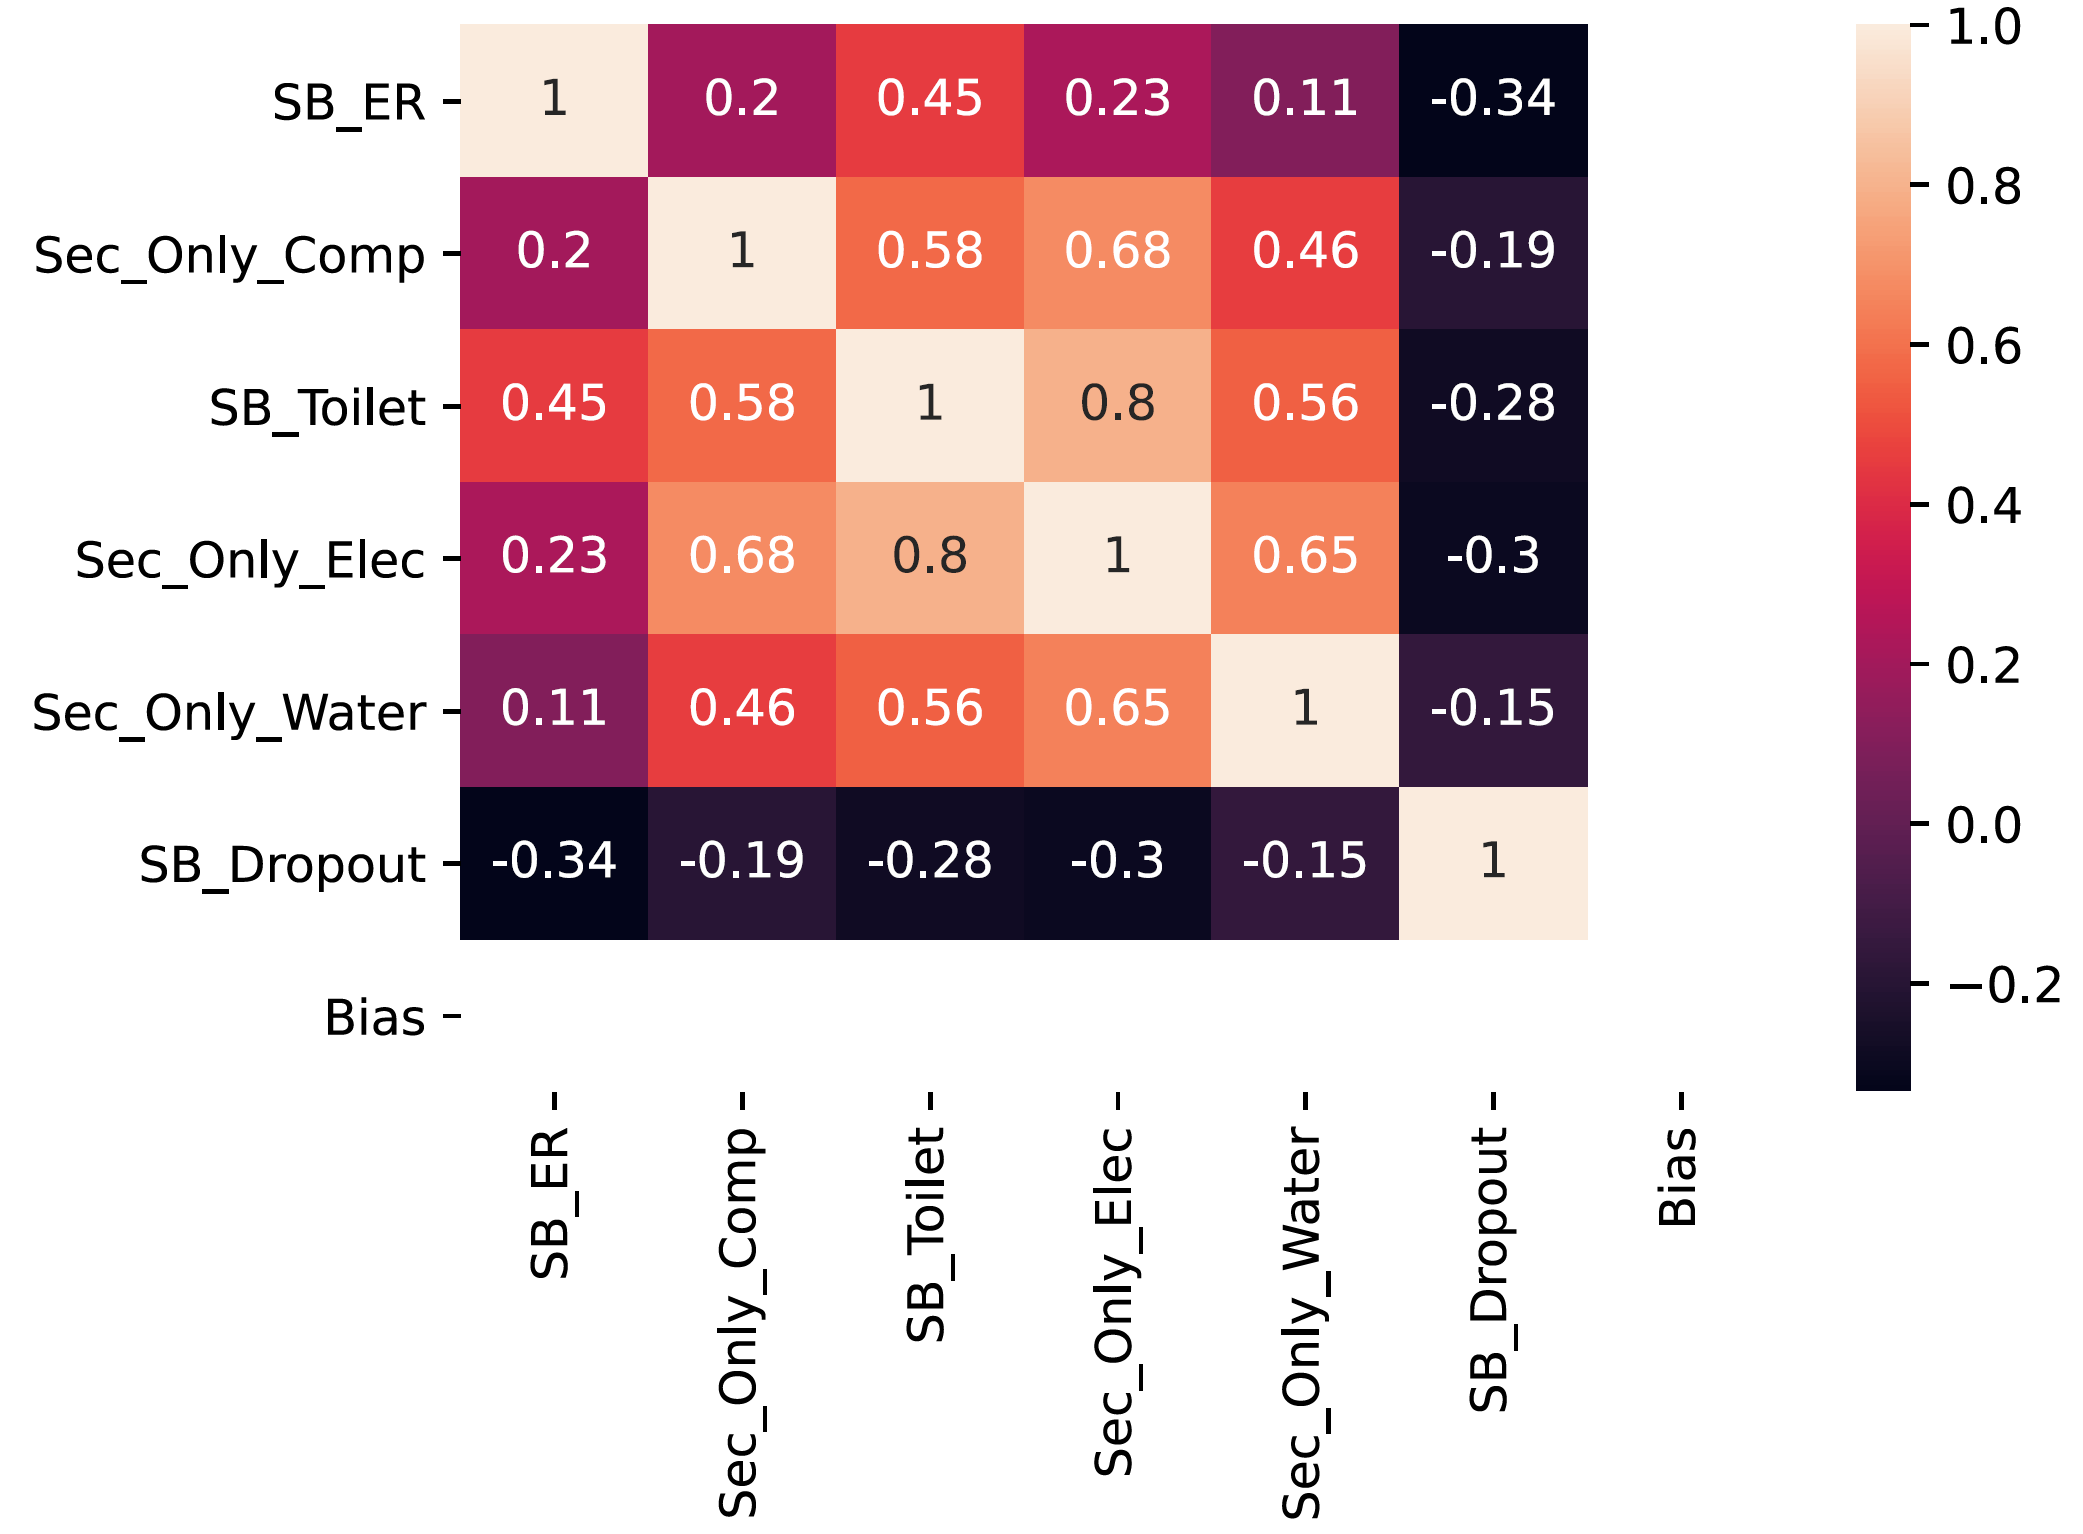
\includegraphics[width=0.4\linewidth]{figures/dropOut_HM_State.png}}
	\subfigure[Histogram]{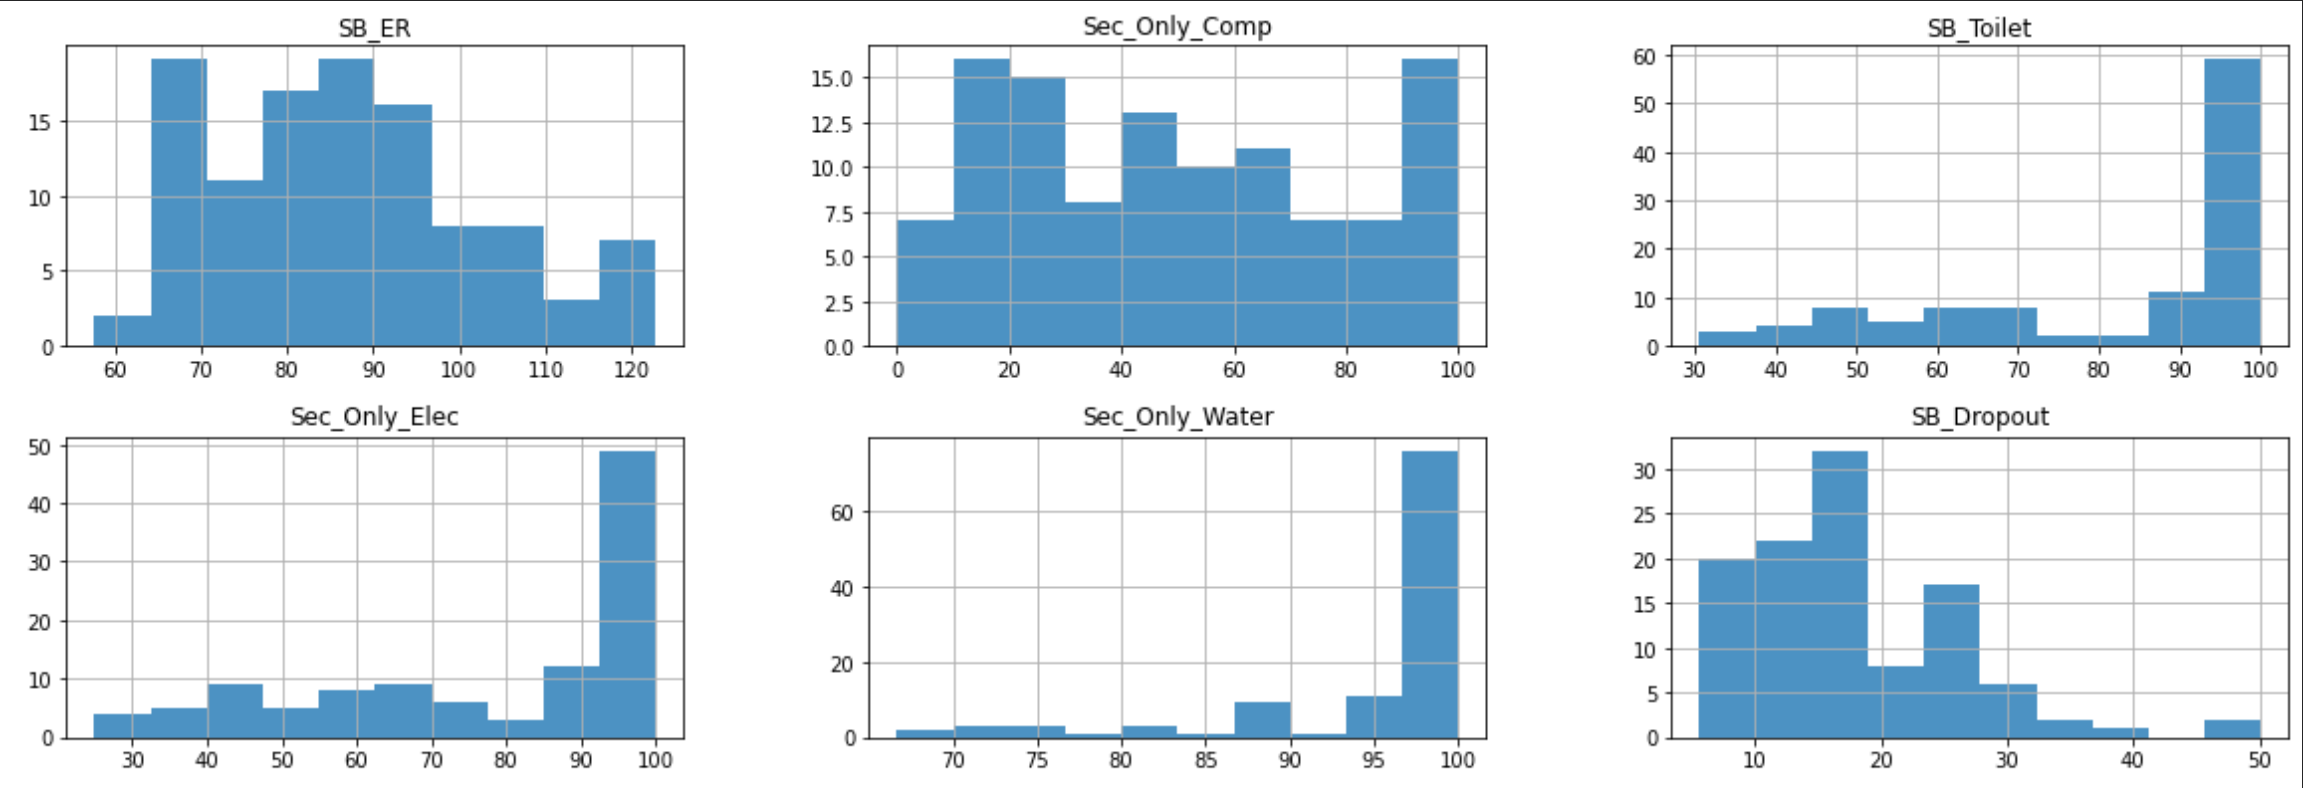
\includegraphics[width=0.5\linewidth]{figures/dropOut_hist_State.png}}
  \caption{State data}
  \label{fig:fig1}
\end{figure}

It is clear from the correlation heatmap that the dropout rates (last row) is dependent on all the chosen features substantially and is negatively correlated.  This is in accordance with the intuition, i.e., if there is higher enrollment, higher number of schools with computers, electricity, toiltes, and drinking water, lower is the dropout rates in that state. Additionally, there appears no high-correlation ($\geq$0.7) amongst the chosen features. 

We used the linear regression codes developed in class for prediction of dropout rates, identification of significant features and providing a confidence interval for the prediction. The results were compared with the outputs from scikit-learn \cite{scikit-learn} using its LinearRegression function for verification purposes.

\subsection{Predicting enrollment rates using linear regression}

The same procedure as mentioned in \hyperref[sec:4.1]{Section 4.1} is repeated with the larger district-level dataset. 
The features in the district-level dataset are: \\
\begin{minipage}[t]{.33\textwidth}
\begin{itemize}
\item Schools with boy's toilets
\item Schools with playground
\item Schools with drinking water
\end{itemize}
\end{minipage}
\begin{minipage}[t]{.33\textwidth}
\begin{itemize}
\item Schools with Roads
\item Classrooms requiring major repair
\item Schools with Electricity
\end{itemize}
\end{minipage}
\begin{minipage}[t]{.33\textwidth}
\begin{itemize}
\item Schools with a single teacher
\item Female literacy rate 
\end{itemize}
\end{minipage}
\\\\
The response was chosen to be the enrollment rate, and the correlation heatmap (Figure \ref{fig:fig2} was studied similarly. 
\begin{figure}[H]
\centering
  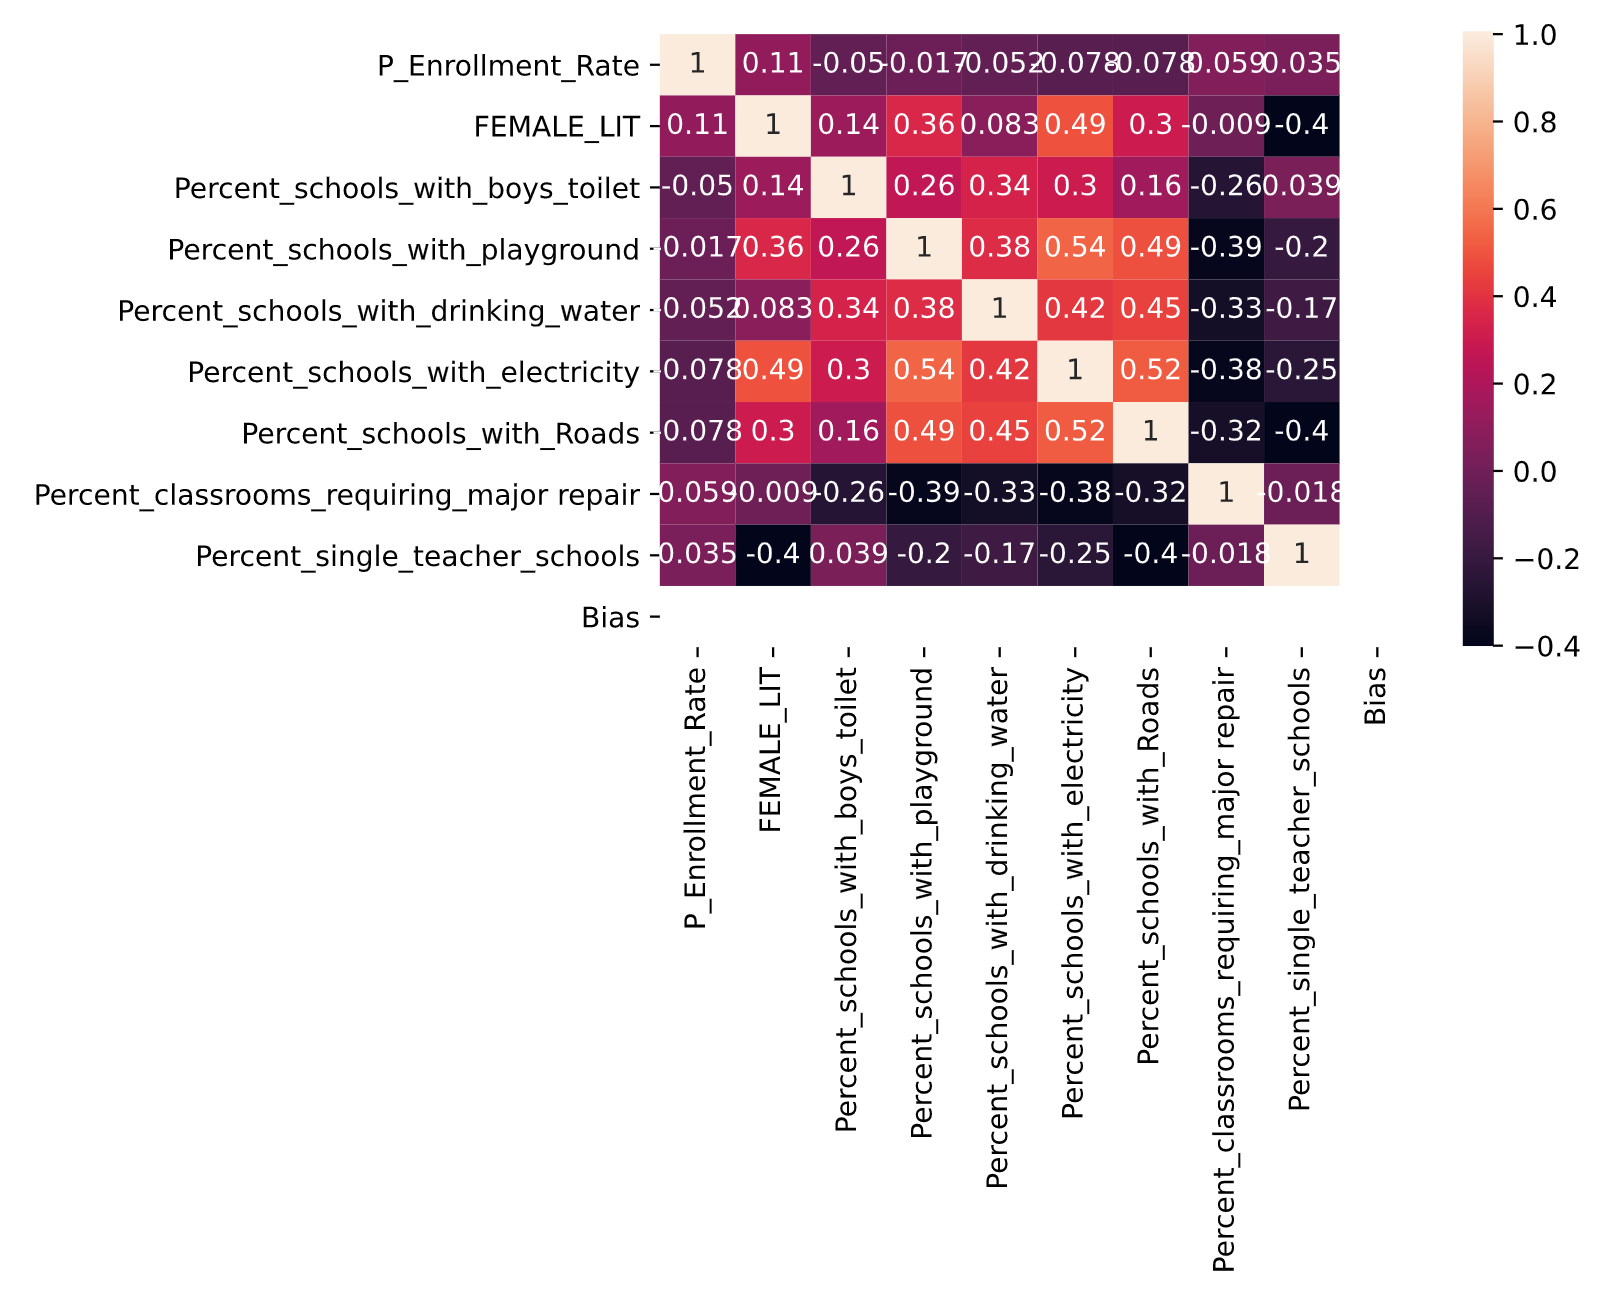
\includegraphics[width=0.75\linewidth]{figures/enroll_HM_Dist.png}
  \caption{Correlation heatmap from district data}
  \label{fig:fig2}
\end{figure}
Some of the correlations made sense, like the enrollment rate was positively correlated with female literacy rate, and negatively correlated with respect to infrastructure related features. However, there were no other significant insights from the chosen features. The linear regression implementation and verification follows the same as \hyperref[sec:4.1]{Section 4.1}.


\subsection{Predicting female literacy rates using Support Vector Machines}
From the correlation matrix shown in Fig.~\ref{fig:fig2}, female literacy rate has a high correlation with many features like percentage of schools with single teachers, percent schools with all-weather roads, percent schools with playground, and percent school with electricity. So we find the effect of other features on the female literacy rate of a district (county). In other words, we predict the female literacy rate as a function of following 6 parameters:\\
\begin{minipage}[t]{.5\textwidth}
	\begin{itemize}
		\item Schools with boy's toilets
		\item Schools with playground
		\item Schools with drinking water
	\end{itemize}
\end{minipage}
\begin{minipage}[t]{.5\textwidth}
	\begin{itemize}
		\item Schools with Electricity
		\item Schools with all-weather roads
		\item Schools with a single teacher
	\end{itemize}
\end{minipage}\\\\
SVM is used as regressor to predict the female literacy rate using Scikit-learn library. K-fold cross validation was conducted.
\begin{itemize}
\item \textbf{Data preprocessing}: The input data was scaled using min-max scaler before feeding to the SVM regressor. Principal component analysis was performed on the input. It showed that all the current features were crucial However, it was found that the number of inputs were already optimum. So none of the features were eliminated.
\item \textbf{Metric used to evaluate the performance}:  It is important to know the correlation between the predicted and actual output. Hence Pearson correlation coefficient (PCC) is better suited and is used in this study to evaluate the performance of the network. It measures the linear correlation between the predicted and true target variable. PCC has values between -1 and +1. +1 indicates positive linear correlation while -1 indicates that variables are negatively correlated. 0 value of PCC indicates the variables are not correlated.   
\item \textbf{Kernel}:  Linear as well as non-linear kernel can be used. Here we used the non-linear `radial basis function' kernel as it is better suited for this data.  
\item \textbf{Best hyperparameters for RBF SVM}:  The performance of RBF SVR depends on the parameters like `gamma' and `C' values. The behavior of the model is sensitive to the gamma parameter. Gamma determines extent of the influence of a single training example.   Also, smaller C provides higher bias and lower variance and vice versa. Best parameters for the model were found by the 'Grid search' function provided by Sklearn. For a given set of gamma and C values, grid search finds the combination which provides the highest score. For this model, the best parameters were: `C': 10, `gamma': 5, with the score of 0.37.
\end{itemize}

\subsection{Predicting female literacy rates using Random Forest}
In order to verify the prediction of SVM, we employ random forest (RF) and NN. RF fits a number of decision trees on the sub-samples of the data to control the over-fitting while improving the accuracy. Data-preprocessing and performance evaluation matrix as mentioned in SVM regressor were used for the random forest model. RF with the following parameters was implemented using `SKLearn' library. Grid search was employed to find the best parameters:  
\begin{itemize}
	\item \textbf{Number of trees in the forest}:  The parameter `n\_estimators' provides this information. Using grid-search, the number of trees selected were 1000. 
	\item \textbf{Quality of split}:  The default parameter 'mean squared error' was used to measure the quality of the split. 
	\item{Minimum number of samples required to split an internal node}: The variable `min\_samples\_split' governs this parameter and was set to 3 by the grid-search.
	\item \textbf{Maximum depth}:  The maximum depth chosen by the Grid-search was `None' which indicated that the RF gave maximum accuracy when the nodes were expanded until all leaves of decision trees are pure or until all leaves contain less than `min\_samples\_split' samples.
\end{itemize}


\subsection{Predicting female literacy rates using Neural Networks}
Data-preprocessing and performance evaluation matrix as mentioned in SVM regressor were used for this neural network (NN) model. NN with following configuration was employed using `keras' library:
\begin{itemize}
	\item \textbf{NN architecture}: In this NN architecture (see Fig.~\ref{fig_NN}a), we gradually increase and then decrease the embedding length of the network so that every layer gains meaningful information from the previous layer and produces relevant embedding. With the input dimension = 6, the first layer has 10 nodes, followed by20-10-5-1 nodes for subsequent layers. The output layer has one node for the target variable. 
	\begin{figure}[h]
		\centering
		\subfigure[Distribution of female literacy rate]{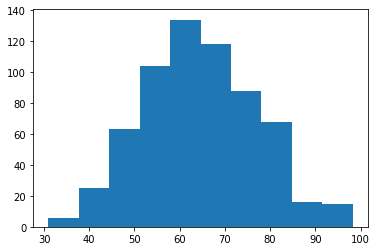
\includegraphics[width=0.4\linewidth]{figures/hist_female_litRate.png}}
		\subfigure[Neural network architecture]{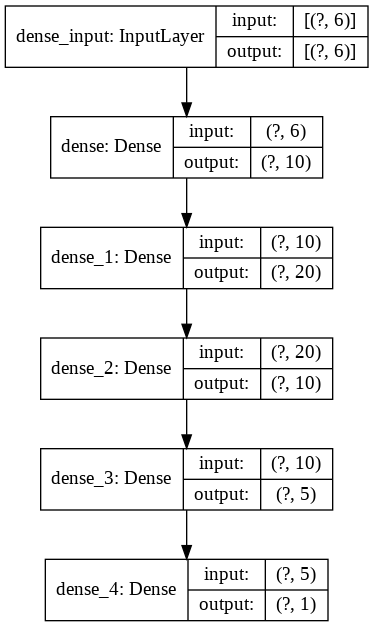
\includegraphics[width=0.2\linewidth]{figures/ann_configuration.png}}
		\caption{State data}
		\label{fig_NN}
	\end{figure}	
	\item \textbf{Activation function}:  Here, we are predicting a continuous numerical value which lies in the range of 0 to 100. `Relu' activation function was used for all the layers. 
	\item \textbf{Optimizer}:  Adams optimizer was used with an adaptive learning rate. It uses a stochastic gradient descent algorithm to minimize the loss function and is based on adaptive estimation of first and second order moments. Adaptive learning rate was employed by as following. The learning rate for the first 2000 epochs was mentained at   $10^{-3}$, and then decreased to $10^{-4}$ for the next 500 epochs. 
	\item \textbf{Loss function}: Popular regression loss functions include: Mean squared error, Mean absolute error,  Mean squared logarithmic  error. Among these, the mean squared logarithmic  error  is suitable if the data has a large spread of values. Values in the present data have a limited spread -- all the values lie between 0 to 100. Moreover, the distribution of the target variable is more or less Gaussian as shown in Fig.~\ref{fig_NN}b, Hence, mean squared error loss function was employed to predict the female literacy rate.   	

\end{itemize}

\section{Results}
\subsection{Prediction of dropout rate(states) and enrollment rate(districts)}
The dropout rate prediction with linear regression is as follows. For feature vector: 
$\xx = 
\begin{bmatrix} 
	100 & 20 & 90 & 90 & 90 
\end{bmatrix} $
The output (dropout prediction) using linear regression are: Predicted dropout rate: 14.105 with confidence interval ($\alpha$ = 0.05): 10.476\% - 17.734\%. Looking at feature significance:
\begin{figure}[H]
\centering
  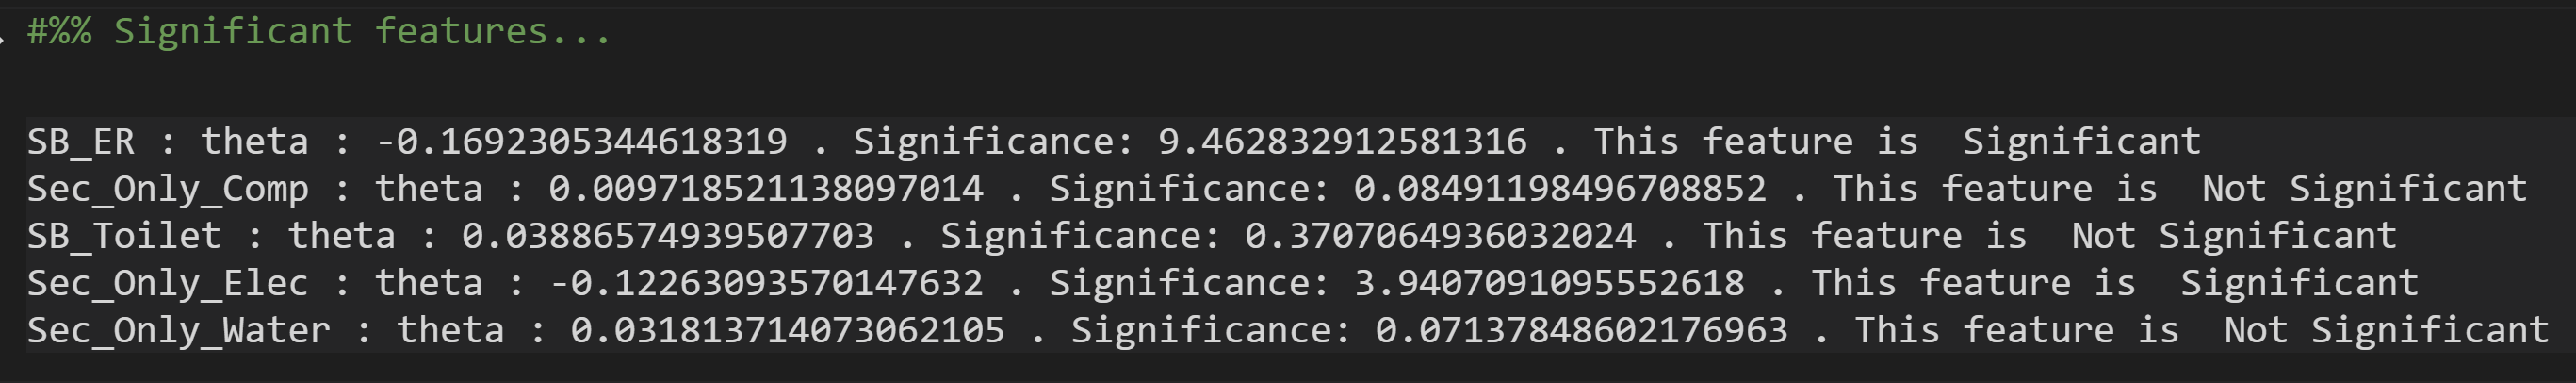
\includegraphics[width=0.6\linewidth]{figures/ResultsDropout2.png}
  \caption{Feature significance for dropout prediction}
  \label{fig:fig5}
\end{figure}
The results and feature significance show that the \textbf{most significant factors influencing dropout rates are the enrollment rates and availability of electricity in schools.} To reduce dropout rates amongst schoolchildren in India, we will need to increase the enrollment rates and increase the number of schools with electricity.\\
%\subsection{Prediction of enrollment rate}
%\subsubsection{With linear regression}
\textbf{Prediction of enrollment rates (districts):} Results from linear regression show that the most significant feature influencing enrollment rate was female literacy rate and the percentage of schools with electricity. The other features showed lower significance. However, the $R^{2}$ values of the fit was not high, close to zero. And a cross-validation score ($\leq40\%$) while predicting within the confidence interval. Thus, linear regression was not the most suitable tool in predicting enrollment rates with these features.
\begin{figure}[H]
\centering
  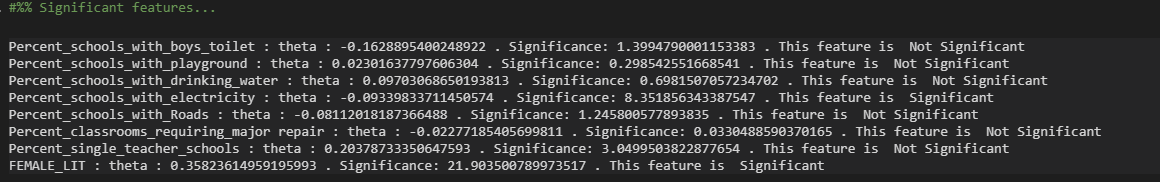
\includegraphics[width=0.6\linewidth]{figures/ResultsEnroll0.png}
  \caption{Feature significance for enrollment prediction}
  \label{fig:fig6}
\end{figure}



\subsection{Prediction of female literacy rate}
\subsubsection{With SVM}
The model was tested and 5-fold cross validation was performed by splitting the data into training and testing sets with the ratio 80:20. Pearson correlation coefficient (PCC)  for the predicted and test data of the target variable `female literacy rate' was obtained as 
\begin{equation*}
\text{PCC}_\text{svm} = 0.5185
\end{equation*} 
For a feature vector: $\xx = 
\begin{bmatrix} 
100 & 20 & 90 & 90 & 90 
\end{bmatrix} $, the predicted female literacy rate by SVM = 63.55
\subsubsection{With Random Forest}
Random forest proves to be a better model compared to SVM for this data providing PCC value of
\begin{equation*}
\text{PCC}_\text{RF} = 0.5936
\end{equation*} 
The plot of predicted and actual values of female literacy rate are shown in the Fig.~\ref{RF_Coorelation}. The values show a good correlation as observed from PCC value as well as the plots. 
\begin{figure}[H]
	\centering
	%	\subfigure[Predicted and actual values  ]{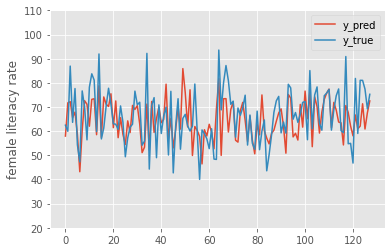
\includegraphics[width=0.4\linewidth]{figures/RF_correlationPlot.png}}
	\subfigure[Predicted and actual values  ]{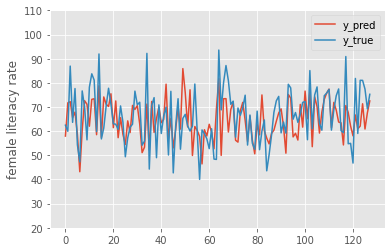
\includegraphics[width=0.35\linewidth]{figures/RF_correlationPlot.png}}
	\subfigure[Scatter plot ]{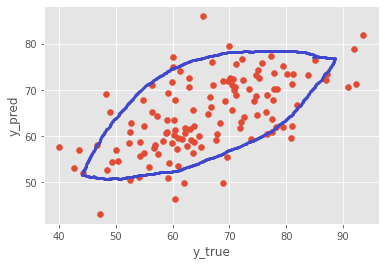
\includegraphics[width=0.35\linewidth]{figures/RF_correlationScatter.png}}
	\caption{Plots of predicted and actual values of target variable for RF}
	\label{RF_Coorelation}
\end{figure}
The blue colored ellipse like outline drawn in Fig.~\ref{RF_Coorelation}b depicts the correlation between the predicted and true values of the target variable. If the outline is narrow and inclined at an angle close to $45^0$, it indicates that the two variables are perfectly correlated. If the outline tends towards a circle, it indicates that the variables are not correlated. Similarly, if is the region is narrow and inclined towards negative $45^0$, it indicates that the variables are negatively correlated. From Fig.~\ref{RF_Coorelation}b, we can see that the variables are positively correlated as expected with the inclination close to $45^0$. 

For the same feature vector, the predicted female literacy rate by RF = 67.43


\subsubsection{With Neural Network}
Next, the NN was implemented for predicting the female literacy rate. The decrease in loss function for various epochs is shown in Fig.~\ref{NN_Coorelation}a. Only 75 epochs are shown in the figure. Actual model was run for more than 2500 epochs. We obtain a higher  PCC value from NN compared to RF and SVM:
\begin{equation*}
\text{PCC}_\text{NN} = \textbf{0.6849}
\end{equation*} 
The scatter plot of predicted and true values of the target variable is shown in Fig.~\ref{NN_Coorelation}c. The red outline (similar to the blue outline in Fig.~\ref{RF_Coorelation}c) indicates the correlation between the two vectors. Compared to Fig.~\ref{RF_Coorelation}c, the outline in the Fig.~\ref{NN_Coorelation}c is narrower which indicates a better correlation between the two vectors. This is reflected in the better PCC value obtained by using NN. 
\begin{figure}[H]
	\centering
	\subfigure[Loss Vs Epoch  ]{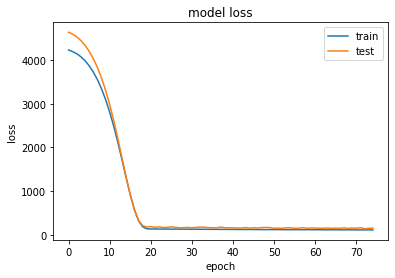
\includegraphics[width=0.3\linewidth]{figures/NN_loss_75.png}}
	\subfigure[Predicted and actual values]{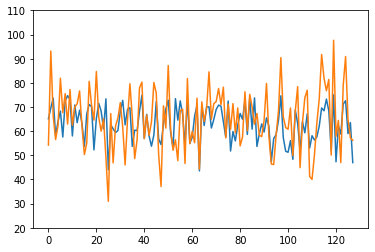
\includegraphics[width=0.3\linewidth]{figures/coorelation.png}}
	\subfigure[Predicted and actual values]{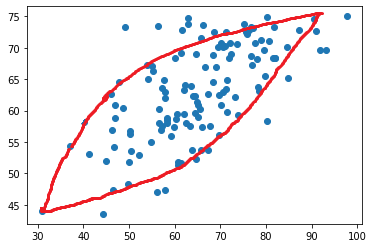
\includegraphics[width=0.3\linewidth]{figures/correlation_scatter_2.png}}
	\caption{Neural network model results}
	\label{NN_Coorelation}
\end{figure}
$R^2$ value obtained for NN model =\textbf{ 0.44}. For the same feature vector, the predicted female literacy rate by NN = 69.40 which is closer to that obtained using RF.
\section{Conclusion and Future Work}
Through this project, we have analyzed few of the factors influencing the dropout rates and enrollment rates amongst the primary schoolchildren in India. Through a linear regression model on the state-wise data, it is seen that dropout rates depend on the enrollment rates and the availability of electricity in schools. It is necessary for the government to increase awareness in enrolling more children to schools and providing basic infrastructure such as electricity. Higher enrollment rates show lower dropouts, thus we attempted to identify what factors affect the enrollment rates amongst children with a district level. We found that enrollment rate is heavily dependent on the female literacy rate of the district and very weakly dependent on the other factors. This supports the fact that female literacy is crucial for encouraging more children to complete their schooling. We further analyzed the factors affecting the female literacy rate in the district. The factors like availability of electricity, clean drinking water, playgrounds, sanitation (availability of toilets) are significant in predicting the female literacy rate. Neural network provided the best accuracy and $R^2$ value followed by random forest and support vector machines. The most significant feature affecting the female literacy is availability of electricity in schools. The second most significant feature is the schools with only one teacher. Many primary schools in India have only one teacher to teach all the subjects for all the classes. Such a ardous work naturally causes strain on the teacher and effects efficiency. If the schools employ more than one teacher, it would help in increasing the female literacy rate. Efforts targeted towards female education through, say more number of evening schools targeted for women, increasing awareness of education among women would bolster the educational system of India.



\pagebreak
\begin{appendices}
\section{Predicting state-wise dropout rates using Linear Regression}
Link to the source dataset: \href{https://www.kaggle.com/vidyapb/indian-school-education-statistics}{Link to Kaggle}. 

CSV data extracted from source link and used for the experiment: \href{https://uwprod-my.sharepoint.com/:x:/g/personal/ssridhara_wisc_edu/Ebu49ou21lVCi4geyN82jpkBzErhT8QkI6XciYx0ed4Cag?e=ExgZ3z}{Click to view CSV}

Code can be downloaded from: \href{https://uwprod-my.sharepoint.com/:u:/g/personal/ssridhara_wisc_edu/EfNbW01wZB1Mof3OfQNlCnsBtZ9gEOjOHpKBEzsP9nn7GA?e=kRUuxN}{Click to download code}
\\
\begin{lstlisting}

#%% ME760 Project - Predicting dropout rates from state-wise education data
import pandas as pd
import numpy as np
import matplotlib.pyplot as plt
from sklearn import linear_model
from sklearn.metrics import mean_squared_error, r2_score
from scipy.stats import norm
from scipy.stats.distributions import chi2

import math

#%%
def read_data(filename):
    df = pd.read_csv(filename)
    df['Bias'] = 1;
    return df

#%%
def linear_regression(my_xvector,df):
    print('Linear regression using own code:')
    y = df['SB_Dropout'].values
    X = df[['Bias','SB_ER','Sec_Only_Comp','SB_Toilet','Sec_Only_Elec','Sec_Only_Water']].values
    theta_hat = np.matmul(np.linalg.inv(np.matmul(X.T,X)),np.matmul(X.T,y));
    N = len(y);
    my_xvector = np.insert(my_xvector, [0], 1);
    y_pred = np.matmul(my_xvector.T, theta_hat);
    print('predicted dropout rate:',y_pred)
    var_hat = (1.0/N)*np.matmul((y - np.matmul(X,theta_hat)).T,(y - np.matmul(X,theta_hat)));
    # print('var_hat',var_hat)
    temp = var_hat*np.matmul(my_xvector.T,np.matmul(np.linalg.inv(np.matmul(X.T,X)),my_xvector));
    tau = norm.ppf(alpha/2,loc = 0,scale = math.sqrt(temp.item(0)))
    # print('tau',tau)
    print('confidence interval:',(y_pred+tau),(y_pred-tau))
    return y_pred
#%%
def LR_significance(my_xvector,df,alpha):
    y = df['SB_Dropout'].values
    Col_names = ['Bias','SB_ER','Sec_Only_Comp','SB_Toilet','Sec_Only_Elec','Sec_Only_Water']
    X = df[Col_names].values

    theta_hat = np.matmul(np.linalg.inv(np.matmul(X.T,X)),np.matmul(X.T,y));
    N = len(y);
    my_xvector = np.insert(my_xvector, [0], 1);
    y_pred = np.matmul(my_xvector.T, theta_hat);

    var_hat = (1.0/N)*np.matmul((y - np.matmul(X,theta_hat)).T,(y - np.matmul(X,theta_hat)));
    # print('var_hat',var_hat)
    temp = var_hat*np.matmul(my_xvector.T,np.matmul(np.linalg.inv(np.matmul(X.T,X)),my_xvector));
    tau = norm.ppf(alpha/2,loc = 0,scale = math.sqrt(temp.item(0)))
    # print('tau',tau)
    # print('confidence interval:',(y_pred+tau),(y_pred-tau))
    #2.7 d and e significant feature height and weight
    cov_theta = var_hat.item(0)*np.linalg.inv(np.matmul(X.T,X));
    # d = 3.841 # from chisquare tables
    cutoff = chi2.ppf(1 - alpha, df=1)

    test_stat_out = np.zeros(len(theta_hat));
    for i in range(1,len(theta_hat)):
        test_stat_out[i] = pow(theta_hat[i]/math.sqrt(cov_theta[i,i]),2)
        if test_stat_out[i] > cutoff:
            is_sig = 'Significant';
        else:
            is_sig = 'Not Significant';
        print(Col_names[i],': theta :',theta_hat[i] ,'. Significance:',test_stat_out[i],'. This feature is ',is_sig)
    return var_hat


#%%
def sk_linear_regression(my_xvector,df):
    print('Using Scikit linearmodel regression')
    y = df['SB_Dropout'].values
    X = df[['SB_ER','Sec_Only_Comp','SB_Toilet','Sec_Only_Elec','Sec_Only_Water']].values
    reg = linear_model.LinearRegression();
    reg.fit(X,y)
    y_pred = reg.predict(my_xvector)

    print('Coefficients: \n', reg.coef_)
    print('Intercept: \n', reg.intercept_)
    

    print('Prediction: \n', y_pred)
    return y_pred
#%% data and histograms
filename = 'school_dataset.csv'
df= read_data(filename)
df.hist(alpha=0.8, figsize=(20, 10))
# ['SB_ER','Sec_Only_Comp','SB_Toilet','Sec_Only_Elec','Sec_Only_Water']
my_xvector = np.array([100,20,90,90,90]).reshape(1, -1);

#%% Predict dropout rate using Scikits Linear regression
# All values in percentage/ratio
y_out = sk_linear_regression(my_xvector,df)
# %% PRedict with Linear regression
y_out = linear_regression(my_xvector,df)
#%% Significant features
alpha = 0.05;
var_hat = LR_significance(my_xvector,df,alpha)
# %%
\end{lstlisting}

\pagebreak
\section{Predicting district-wise enrollment rate using Linear Regression}
Link to the source dataset: \href{https://www.kaggle.com/rajanand/education-in-india}{Link to Kaggle}. 

CSV data extracted from source link and used for the experiment: \href{https://uwprod-my.sharepoint.com/:x:/g/personal/ssridhara_wisc_edu/EZXFqgkG02BKhupEidEdMzwBQxlku7ZHe6UGNOKJ_DWt9A?e=89GG2G}{Click to view CSV}

Code can be downloaded from: \href{https://uwprod-my.sharepoint.com/:u:/g/personal/ssridhara_wisc_edu/ERE1fkFjT1tPvzMqik46o1UBbDBkdWNj7p3jxP4TITbzuw?e=UcE0cs}{Click to download code}\\

\begin{lstlisting}

#%% ME760 Project - Predicting enrollment rates from district-wise education data
#%%
import pandas as pd
import numpy as np
import matplotlib.pyplot as plt
from sklearn import linear_model, metrics
from sklearn.metrics import mean_squared_error, r2_score
from sklearn.model_selection import  cross_val_score
from sklearn.model_selection import train_test_split
from scipy.stats import norm
from scipy.stats.distributions import chi2
import seaborn as sn

import math

#%%
def read_data(filename):
    df = pd.read_csv(filename)
    df['Bias'] = 1;
    return df
#%%
def read_data_with_fields(filename,fields):
    df = pd.read_csv(filename,usecols = fields)
    df['Bias'] = 1;
    return df
#%%
def linear_regression(my_xvector,df,alpha,fields):
    # print('Linear regression using own code:')
    y = df[fields[0]].values
    # fields.insert(1,'Bias')
    Col_names = fields[1:len(fields)]   
    X = df[Col_names].values
    theta_hat = np.matmul(np.linalg.inv(np.matmul(X.T,X)),np.matmul(X.T,y));
    print(theta_hat)
    N = len(y);
    my_xvector = np.insert(my_xvector, [0], 1);
    y_pred = np.matmul(my_xvector.T, theta_hat);
    # print('predicted enrollment rate:',y_pred)
    var_hat = (1.0/N)*np.matmul((y - np.matmul(X,theta_hat)).T,(y - np.matmul(X,theta_hat)));
    # print('var_hat',var_hat)
    temp = var_hat*np.matmul(my_xvector.T,np.matmul(np.linalg.inv(np.matmul(X.T,X)),my_xvector));
    tau = norm.ppf(alpha/2,loc = 0,scale = math.sqrt(temp.item(0)))
    # print('tau',tau)
    # rint('confidence interval:',(y_pred+tau),(y_pred-tau))
    y_lb = y_pred+tau
    y_ub = y_pred-tau
    return y_pred,y_lb, y_ub
#%%
def LR_significance(my_xvector,df,alpha,fields):
    y = df[fields[0]].values
    # fields.insert(1,'Bias')
    Col_names = fields[1:10]   
    X = df[Col_names].values

    theta_hat = np.matmul(np.linalg.inv(np.matmul(X.T,X)),np.matmul(X.T,y));
    N = len(y);
    my_xvector = np.insert(my_xvector, [0], 1);
    y_pred = np.matmul(my_xvector.T, theta_hat);

    var_hat = (1.0/N)*np.matmul((y - np.matmul(X,theta_hat)).T,(y - np.matmul(X,theta_hat)));
    # print('var_hat',var_hat)
    temp = var_hat*np.matmul(my_xvector.T,np.matmul(np.linalg.inv(np.matmul(X.T,X)),my_xvector));
    tau = norm.ppf(alpha/2,loc = 0,scale = math.sqrt(temp.item(0)))
    # print('tau',tau)
    # print('confidence interval:',(y_pred+tau),(y_pred-tau))
    #2.7 d and e significant feature height and weight
    cov_theta = var_hat.item(0)*np.linalg.inv(np.matmul(X.T,X));
    # d = 3.841 # from chisquare tables
    cutoff = chi2.ppf(1 - alpha, df=1)

    test_stat_out = np.zeros(len(theta_hat));
    for i in range(1,len(theta_hat)):
        test_stat_out[i] = pow(theta_hat[i]/math.sqrt(cov_theta[i,i]),2)
        if test_stat_out[i] > cutoff:
            is_sig = 'Significant';
        else:
            is_sig = 'Not Significant';
        print(Col_names[i],': theta :',theta_hat[i] ,'. Significance:',test_stat_out[i],'. This feature is ',is_sig)
    return var_hat


#%%
def sk_linear_regression(my_xvector,df,fields):
    print('Using Scikit linearmodel regression')
    y = df[fields[0]].values
    X = df[fields[2:len(fields)]].values
    reg = linear_model.LinearRegression();
    reg.fit(X,y)
    y_pred = reg.predict(my_xvector)

    print('Coefficients: \n', reg.coef_)
    print('Intercept: \n', reg.intercept_)
    

    print('Prediction: \n', y_pred)
    return y_pred


#%% 
def LR_CV(df,n_folds,alpha,fields):
    fold_size = math.floor(len(df)/n_folds)
    list_of_dfs = [df.loc[i:i+fold_size-1,:] for i in range(0, len(df),fold_size)]
    error_count = 0;
    for i in range(n_folds):
        test_df = list_of_dfs[i]
        train_df = df.drop(df.index[test_df.index[0]:test_df.index[-1]])
        j = 0;
        for j in range(len(test_df)):
            truth = test_df.values[j][0];
            prediction, pred_lb, pred_ub = linear_regression((test_df.values[j][2:len(fields)]), train_df, alpha, fields);
            if(pred_lb <= truth <= pred_ub):
                # print('Me here')
                error_count += 0;
            else:
                # print('Me here')
                error_count += 1;
    CV_out = 100*(1-(error_count/len(df)));
    print('Accuracy with cross-validation =',CV_out);
    return CV_out

#%%
def LR_CV2(df, fields, n_folds):
    y = df[fields[0]].values
    X = df[fields[2:len(fields)]].values
    X_train, X_test, y_train, y_test = train_test_split(X, y, test_size=0.20, random_state=0)
    reg = linear_model.LinearRegression() 
    reg.fit(X_train, y_train)
    scores = cross_val_score(reg, X_train, y_train, cv = n_folds)
    print("mean cross validation score: {}".format(np.mean(scores)))
    print("score without cv: {}".format(reg.score(X_train, y_train)))
    
    y_pred = reg.predict(X_test)
    print('R2 score:',r2_score(y_test, y_pred))
    print('regressor score:',reg.score(X_test, y_test))
    print('Mean Absolute Error:', metrics.mean_absolute_error(y_test, y_pred))
    print('Mean Squared Error:', metrics.mean_squared_error(y_test, y_pred))
    print('Root Mean Squared Error:', np.sqrt(metrics.mean_squared_error(y_test, y_pred))) 
#%% correlation analysis
filename = 'Reduced_data_district_2.csv'
df= read_data(filename)
df = df[df.P_Enrollment_Rate.notnull()]
df.P_Enrollment_Rate = pd.to_numeric(df.P_Enrollment_Rate, errors='coerce')
df = df.dropna()
corrMatrix = df.corr()
# sn.heatmap(corrMatrix, annot=True)
sn.heatmap(corrMatrix, vmax=0.9, square=True)
plt.show()



#%% data and histograms
filename = 'Reduced_data_district_2.csv'
fields =['P_Enrollment_Rate','Percent_schools_with_boys_toilet','Percent_schools_with_playground',\
        'Percent_schools_with_drinking_water','Percent_schools_with_electricity',\
            'Percent_schools_with_Roads','Percent_classrooms_requiring_major repair','Percent_single_teacher_schools','FEMALE_LIT'];
df= read_data_with_fields(filename,fields)
df = df[df.P_Enrollment_Rate.notnull()]
df.P_Enrollment_Rate = pd.to_numeric(df.P_Enrollment_Rate, errors='coerce')
df = df.dropna()
fields.insert(1,'Bias')
# df.hist(alpha=0.8)
my_xvector = np.array([65,60,96,57,87,9,7,20]).reshape(1, -1);
alpha = 0.05;
corrMatrix = df.corr()
sn.heatmap(corrMatrix, annot=True)
plt.show()




#%% Predict dropout rate using Scikits Linear regression
y_out,y_lb,y_ub = linear_regression(my_xvector,df,alpha,fields)
#%% using SKlearn
# All values in percentage/ratio
y_out = sk_linear_regression(my_xvector,df,fields)
# %% PRedict with Linear regression
# y_out = linear_regression(my_xvector,df)
#%% Significant features
var_hat = LR_significance(my_xvector,df,alpha,fields)


# %% Cross validation of linear regression
n_folds = 5;
CV_out = LR_CV(df,n_folds,alpha,fields);


# %%
LR_CV2(df, fields, n_folds)
# %%

\end{lstlisting}


\pagebreak
\section{Predicting district-wise enrollment rate using Support Vector Machines and Random Forest}
\begin{lstlisting}

#%% ME760 Project - Predicting female literacy rate from district-wise education data
#%%
import numpy as np
import pandas as pd
import csv
import math
from sklearn.svm import SVR
from sklearn.model_selection import KFold
from sklearn.model_selection import GridSearchCV
from sklearn.metrics import r2_score
from sklearn.metrics import mean_squared_error 
from sklearn.preprocessing import MinMaxScaler
from sklearn.decomposition import PCA
import matplotlib
from matplotlib import pyplot as plt
matplotlib.style.use('ggplot')
import scipy
from sklearn.model_selection import train_test_split
from scipy.stats import pearsonr
from sklearn.ensemble import RandomForestRegressor

def read_data_with_fields(filename,fields):
df = pd.read_csv(filename,usecols = fields)
return df

filename = 'Reduced_data_district_2.csv'
fields =['FEMALE_LIT','Percent_schools_with_boys_toilet','Percent_schools_with_playground',\
'Percent_schools_with_drinking_water','Percent_schools_with_electricity','Percent_schools_with_Roads', 'Percent_single_teacher_schools']
df= read_data_with_fields(filename,fields)

df = df.dropna()

y = df[fields[0]].values
X = df[fields[1:7]].values
X_train, X_test, y_train, y_test = train_test_split(X, y, test_size=0.20, random_state=0)

sc= MinMaxScaler()
X_train = sc.fit_transform(X_train)
X_test = sc.transform(X_test)

kf = list(KFold(n_splits=5).split(X_train,y_train))

#SVR

C_range = [0.001, 0.01, 0.1, 1, 5, 10]
gamma_range = [0.001, 0.01, 0.1, 1, 5, 10]
kernel_range = ["rbf"]

param_grid = dict(gamma=gamma_range, C=C_range, kernel=kernel_range)

grid = GridSearchCV(SVR(), param_grid=param_grid, cv=kf, n_jobs=1, verbose=1)
grid.fit(X_train, y_train)
print("The best parameters are %s with a score of %0.2f"% (grid.best_params_, grid.best_score_))

reg_svr = SVR(C=grid.best_params_['C'], gamma=grid.best_params_['gamma'])
reg_svr.fit(X_train, y_train)
y_pred = reg_svr.predict(X_test)
print('correlation:', pearsonr(y_test, y_pred))

import matplotlib.pyplot as plt
plt.ylim(20, 110)

plt.plot(reg_svr.predict(X_test))
plt.plot(y_test)

plt.scatter(y_test,reg_svr.predict(X_test))

print('correlation:', pearsonr(y_test, y_pred))

my_xvector =  np.array([65,60,96,57,87,7]).reshape(1, -1);
my_xvector = sc.fit_transform(my_xvector)
y_out = reg_svr.predict(my_xvector)
y_out

#Random Forest

param_grid = {'n_estimators': [500, 700, 1000], 'max_depth': [None, 1, 2, 3], 'min_samples_split': [2, 3]}
grid = GridSearchCV(RandomForestRegressor(), param_grid=param_grid, cv=kf, n_jobs=1, verbose=1)
grid.fit(X_train, y_train)
print("The best parameters are %s with a score of %0.2f"% (grid.best_params_, grid.best_score_))

clf = RandomForestRegressor(n_estimators=grid.best_params_['n_estimators'], max_depth=grid.best_params_['max_depth'], min_samples_split=grid.best_params_['min_samples_split'])
clf.fit(X_train, y_train)
y_pred = clf.predict(X_test)
print('correlation:', pearsonr(y_test, y_pred))

import matplotlib.pyplot as plt
plt.ylim(20, 110)
plt.plot(clf.predict(X_test))
plt.plot(y_test)
plt.ylabel('female literacy rate')
labels = ['y_pred','y_true']
plt.legend(labels)
plt.scatter(y_test,clf.predict(X_test))
plt.ylabel('y_pred')
plt.xlabel('y_true')

my_xvector =  np.array([65,60,96,57,87,7]).reshape(1, -1);
my_xvector = sc.fit_transform(my_xvector)
y_out = clf.predict(my_xvector)


\end{lstlisting}
\pagebreak
\section{Predicting district-wise enrollment rate using Artificial Neural Networks}
\begin{lstlisting}

#%% ME760 Project - Predicting female literacy rate from district-wise education data
#%%
import pandas as pd
import numpy as np
import matplotlib.pyplot as plt

# import the regressor 
from sklearn import metrics
from sklearn.model_selection import  cross_val_score
from sklearn.model_selection import train_test_split
from sklearn.metrics import r2_score

from keras.models import Sequential
import keras
from keras.layers import Dense
from sklearn.model_selection import KFold
from sklearn.datasets import make_regression
from sklearn.preprocessing import MinMaxScaler
from numpy import array
from sklearn.preprocessing import  MinMaxScaler
import matplotlib.pyplot as plt
from sklearn.metrics import mean_squared_error
from scipy.stats import pearsonr

def read_data_with_fields(filename,fields):
df = pd.read_csv(filename,usecols = fields)
return df

# data
filename = 'Reduced_data_district_2.csv'
fields =['FEMALE_LIT','Percent_schools_with_boys_toilet','Percent_schools_with_playground',\
'Percent_schools_with_drinking_water','Percent_schools_with_electricity','Percent_schools_with_Roads', 'Percent_single_teacher_schools']
df= read_data_with_fields(filename,fields)

df = df.dropna()
y = df[fields[0]].values
X = df[fields[1:7]].values

X_train,X_test,y_train,y_test = train_test_split(X,y,test_size = 0.2,random_state = 1)

sc= MinMaxScaler()
X_train = sc.fit_transform(X_train)
X_test = sc.transform(X_test)

model = Sequential()
model.add(Dense(10, input_dim=6, activation='relu'))
model.add(Dense(20,  activation='relu'))
model.add(Dense(10,  activation='relu'))
model.add(Dense(5,  activation='relu'))
model.add(Dense(1, activation='linear'))

keras.optimizers.Adam(lr=0.0001, beta_1=0.9, beta_2=0.999, amsgrad=False)
model.compile(loss='mean_squared_error', optimizer='RMSprop', metrics=['mean_absolute_percentage_error', 'mse'])

history = model.fit(X_train, y_train, epochs=2000, batch_size=32,validation_split=0.15,validation_data=None,verbose=1)

plt.ylim(60, 110)
plt.plot(model.predict(X_test))
plt.plot(y_test)
plt.ylim(60, 110)
plt.plot(model.predict(X_train))
plt.plot(y_train)

y_pred = np.concatenate(model.predict(X_test)).ravel().tolist()

y_true = y_test.ravel().tolist()


print(PCC = pearsonr(y_pred, y_true))

# summarize history for loss
plt.plot(history.history['loss'])
plt.plot(history.history['val_loss'])
plt.title('model loss')
plt.ylabel('loss')
plt.xlabel('epoch')
plt.legend(['train', 'test'], loc='upper right')
plt.show()

my_xvector =  np.array([65,60,96,57,87,7]).reshape(1, -1);
my_xvector = sc.fit_transform(my_xvector)

y_out = model.predict(my_xvector)

\end{lstlisting}

\pagebreak
\end{appendices}

\bibliography{my_bib}
\end{document} 
































